\chapter{Neural Network}
Neural Network is used to study and model biological systems and learning processes (used in Philosophy, Psychology and neurobiology, cognitive science, Computational neuroscience).
We use Neural Network to introduce effective ML systems/algorithms, often losing a strict biological realism, and that is concern on Statistics, Artificial Intelligence, Physics, Math., Engineering, and where ML, computational  and algorithmic properties are essential.

We will analyze in this course \emph{ANN (Artificial Neural Networks)} is indeed a (flexible) Machine Learning tool (in the sense of approximation of functions:
it realizes a mathematical functions h(x) with special properties), infact NN can learn from examples, are a universal approximators (Theorem of Cybenko: flexible approaches for arbitrary functions),
can deal with noise and incomplete data (Performance degrade gracefully under adverse operating conditions), and in the end NN can handle  continuous real and 
discrete data for both regression and classification tasks.\newline
NN is a successful model in ML due to the flexibility in applications and encompasses a wide set of models, so it is a paradigm (in the class of subsymbolic approaches).

Each node in NN is called neuron or unit (see figure \ref{img:neuron}) and the input are from extern source or other units (IR) and the connection is done by weight w
(free parameters, that can be modified by learning (synaptic strength)), where we have that the weighted sum $net_i$ is called the net input to unit $i$,defined as 
\[ net_i(x) = \sum _j w_{ij} x_j \]
and note that $w_{ij}$ refers to the weight of the unit $i$ and the function $f$ is the unit's activation function(e.g linear, LTU, ...), where the result
of $f(net_i)$ is the output $o_i$ of a node $i$.

\begin{figure}
    \caption{Structure of ANN node}
    \label{img:neuron}
    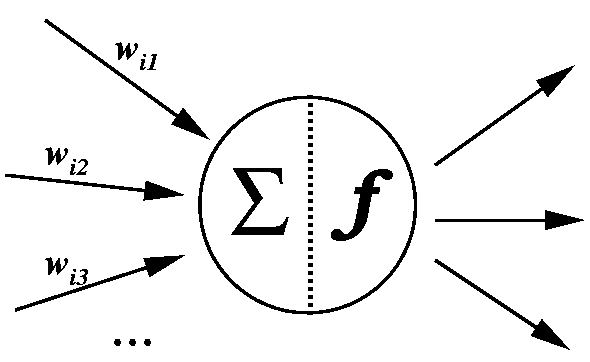
\includegraphics[width=\textwidth]{images/artificialNeuron}
\end{figure}
Every Boolean function can be represented by some network of interconnected perceptrons, only two levels deep is sufficient (or more can be more efficient*), but single layer 
cannot model all the possible functions, like for example XOR function, so we need hidden layers in NN to represent complex tasks.

There are two kinds of method for learning:
\begin{description}
    \item[Adaline (Adaptive Linear Neuron invented by Widrow, Hoff):] linear, LMS direct solution and gradient descent solution, as we have introduced in Regression and Classification chapter,
	    							      that is not proved to converge but only with an approximation.
    \item [Perceptron(Rosenblatt):] non-linear (with hard limiter or Threshold activation function) and can be used only for classification and it is ensured that converge.
	    			    Perceptron represent linear decision boundaries, can solve only linearly separable problems and it has as activation function the following
				    \[ f = sign(\transpose{\theta}x) \]
				    with values that can be $1$ (positive class) or $-1$ (negative class).
					
				   Perceptron learning algorithm consist to compute the predicted output $out = sign(\transpose{\theta}x)$ and if $out \neq y$ we update the weights $\theta$ using
				   \[ \theta = \theta + \frac{1}{2} \eta (y - sign(\transpose{\theta}x)) x \]

				   \begin{thm}
					   Perceptron is guaranteed to converge (classifying correctly all the input patterns) in a finite number of steps if the problem is linearly separable.
				   \end{thm}
\end{description}
Common activation function are the linear, logistic, $\tanh$ function but it is also used the softmax function, RELU(Rectified Linear Unit) and gaussian function,
anyway usually we will use a different activation between output and hidden units and common choice are $\tanh$ for hidden unit and linear for output unit.

We will analyze standard feedforward NN, where the architecture of a NN defines the topology of the connections among the units and the two-layer feedforward neural network 
described in \ref{img:feedforward} and \ref{img:feedEquation}, corresponds to the well-know MLP(Multilayer Perceptron) architecture: the units are connected by weighted links 
and they are organized in the form of layers. 

The Hypothesis space of feedforward NN is the continuous space of all the functions that can be represented by assigning the weight values of the given architecture and many early results
(Cybernko 1989 and so on) estabilish that a single hidden-layer network (with logistic activation functions) can approximate (arbitrarily well) every continuous (on hyper cubes) function
(provided enough units in the hidden layer) so a MLP network can approximate (arbitrarily well) every input-output mapping (provided enough units in the hidden layers).

The univ.approx. theorem is a fundamental contribution•It show that 1 hidden layer is sufficient in general, but it does notassure that a “small number” of units could be sufficient (it does not provide a limit on such number)•It is possible to find boundaries on such number (for many f. families)•But also to find “no flattening” results (on efficiency, not expressivity):–cases for which the implementation by a single hidden layer would require an exponential number of units (w.r.t n input dim.), or non-zero weights,–while more layers can help (it can help for the number of units/weights and/or for learning such approximation)–But is it easy to optimize (training) a MLP with many layers

NN with backprogationlearning algorithm: •Generally related to the smoothnessproperties of functions:–Small input variations small output variations–E.g. a locally limited value of the first derivative.–A very common assumption in ML•Why make sense? A target function that is not Non-smooth: random number generator generalization cannot be achieved

The learning algorithm allows adapting the free-parameters wof themodel, i.e. the values of the connection-weight, in order to obtain the best approximationof the target function. •In the ML framework this is often realized in terms of minimizationof an error (or loss) function on the training data set.•The problem is the same we have seen for the other models (repetita), starting again with the simple LMS case:–Givena set of ltraining example  (xp,dp)  and a loss function (measure) L –Find: The weight vector wthat minimizes the expected loss on the training data:

Note that in general:•Loading problem: (“loading” a given set of tr data into the free par. of the NN) –given a network and a set of examples –answer yes/no: is there a set of weights so that the network will be consistent with the examples?•The loading problem is NP-complete (Judd, 1990)•This implies that hard problems cannot be “solved” ! •In practice networks can be trained in a reasonable amount of time (see the back prop alg.) although optimal solution is not guaranteed

Find  w by computing the gradient of the error (loss) function•Epoch: an entire cycle of training pattern presentation•Nice properties (also for programming):–easy because of the compositional form of the model–keep track only of quantities local to each unit (by local variables) modularityof the units is preserved

To train an multilayer feedforward NN it has been introduced in \cite{backpropagation} the \emph{Backpropagation} algorithm, that it is an evolution
BACKPROPAGATION

General problems:•The model is often over-parametrized•Optimization problem is not convex and potentially unstable

Hyper-parameters= values that youhave to set-up to run the training

Starting values (winitialin the basic alg.)•(!)Initialize weights by random values near zero –Avoid for W: all zero, high values, or all equals (symmetry): these can hamper the training•E.g. in the range [-0.7,+0.7] (for standardized data, see later)•Considering the Fan-in : e.g. range * 2/fan-in–Not if fan-in is too large–Not for output units (else delta start close to zero !)•Other heuristics ...orthogonal matrix, .... (enjoy if  you like) –Very popular among practitioners: Glorot, BengioAISTATS 2010: 0 for biases and w random from Uniform distribution in [-1/a, +1/a] with a=sqrt(fan-in) or (later results) a depending also on fan-out ... •Note (practicalfor the first part of the project): a very small NN (very few units) can have a stronger dependencies w.r.t.initialization

Multiple Minima•Loss is not convex: many local minima•The result depends on starting weight values•Not really a big issue –you can see the final training error–a “good” local minima is often sufficient (see the next slide)•(!)Try a number of random starting configurations(e.g. 5-10 or more training runs or trials)•Take the mean results (mean of errors) and look to varianceto evaluateyour model and then, if you like to have only 1 response :–you can choose the solution giving lowest (penalized) error (or the median)–You can take advantage of different end points by an average (committee) response: mean of the outputs/voting

ndeed in ML we don’t need neither local or global minima on Rempas we are searching the min of R(that we cannot compute). –Often we stop in a point that has not null gradient and hence also  neither a local or global minima for the empirical (training) error.•The NN build a variable size hpspace (see at the end of NN-first part slides)→it increases VC-dim during training →the training  error decreases toward zero not because we reach a global minimum but because the NN becomes too complex (high VC-dim)•Stopping before this condition of overtraining(and hence overfitting) is needed

For Batch version: sum up all the gradients of each pattern over an epoch and then update the weights (Dwafter each “epoch” of lpatterns)•Stochastic/on-lineversion: upgrade wfor each pattern p (by Dpw)  without wait the total sum over l:–It makes progress with each examples it looks at: it can be faster, but it need smaller eta

Batch version: more accurate estimation of gradient •On-line or Stochastic version:  since the gradient for a single data point can be considered a noisy approximation to the overall gradient, this is also called stochastic(noisy) gradient descent. Zig-zag (stochastic) descent (see figures in the next slide)–It can help avoiding local minima–A different order of patterns in different epochs should be used  (to avoid a bias/drift in the gradient descending)–(!)Usually random order (shuffling the patterns)•Many variationsexist: for instance –Stochastic Gradient Descent (SGD) using minibatch –mb (few training examples) for each step of gradient descent

Minibatchstochastic method →akaSGD–Use random sampling to implement the minibatch(unbiased estimation). By shuffling  (at the beginning for all the TR data or for each mini batch)–With very large TR set or online streaming →even no epochs!–Along with the advantage of gradient descent (linear cost wrtexamples) SGD with mbis a key factor in extending learning to very large data sets (over millions of examples) because mb(and hence the cost of each SGD update) does not depend on l : typically just mini-batch  and  (again) no epochs repetition

Batch: more accurate estimation of gradient →higher eta value•On-line:it can make the training faster but can be more unstable →smaller eta valueMore in general (on the eta values):•High versuslow etavalues :  fast (but possible unstable if too large) versusstable (but possible too slow if too small)•And we will see various techniques to improve the convergence speed•Anyway, still you ask for some values ?!?Typically, search in the range [0.01-0.5] in LMS

Learning curve, plotting errors during training, it allows you to check the behavior in the early phases of the model design for your task at hand (preliminary trials)–Please check the Learning Curve whiletraining a NN! •We are now looking to the curve quality and convergence speed: of course the absolute value for the training error depends also on the model capacity (see later for the number of units, regularization etc.) and the other hyperparameters

Practical approach: it is useful to use of the mean(average) of the gradients over the epoch: it helps to have an “uniform” approach with respect to the number of input data
Repetitafrom “Gradient descent algorithm”: dividing by l  correspond to have the LeastMeanSquares–Note that it is equivalent to  have: eta/l–Off course divide by mb for mini batch•Note that if you compare on-line with batch using LMS (i.e. /l), then using on-line training will require much smaller eta to be comparable!!!! (in order of the same factor /l used to divide the gradient in the batch version

Momentum –NesterovMomentum2.Variable learning rate (initially high then decrease)3.Adaptive learning rates (change during training and for each w) (see also in Deep Learning  lectures)4.In NN with many layers (see deep learning lectures): –It can be varied depending on the layer (higher for deep layers) or fan-in (higher for few input connections)

Faster in plateaus: same sign of grad. for consecutive iterations →momentum increase the delta •Damps oscillations: stabilizing effect in directions that oscillate in sign•Inertia effect: Allow us to use higher eta (learning parameter: e.g. 0.2-0.9)
Alfa: 0<momentum parameter <1 e.g 0.5 -0.9

Effect on a canyon of the error surface (#poor conditioning of the Hessian matrix).•In redthe path with the momentum, lengthwise traversing the valley toward the minimum•Instead of zig-zag along the canyon walls (following the blackdirections given by the gradient)

Momentum born with “batch” learning, and it is commonly assumed that helps more in  batch mode •In the on-lineversion can be used but it is connected to a moving average of the past gradients concept to smooth out the stochastic gradient samples [e.g. see it in the form grad= alfa grad+(1-alfa) gradnow]•It smooths the gradient over different examples (a different meaning w.r.t.the batch version that uses the same batch of examples)•You can use it multiplying by eta (as usual) to obtain the  DeltaW

For Minibatch: moving average of past gradients over the progressive minibatchs(that have different examples, not the step before for the same examples as for batch)

Using mini-batch →the gradient does not decrease to zero close to a minimum (as the exact gradient can do)•Hence fixed learning rate should be avoided:•For instance, we can  decay linearly eta for each step until iteration tau (), using =(step s)/:•Then stop and use fix (small) •Set-up: as ~1% of 0, few hundred steps•And 0 ? Again: no instability/ no stuck trade-off (preliminary trials or grid-search

Adaptive Learning Rates•Automatically adapt the learning rate during training•Possibly avoiding/reducing the fine tuning phase via hyperparameters selection•Use separate etafor each parameter

As any iterative approaches.... Basic SGD is generally efficient (linear in the number of free parameters)  but depends on the number of training data and on the number of epochs

Use the second order derivatives (Hessian matrix): more information about the curvature of the objective function →better descent (Newton's methods )–But the Hessian can be too large (i.e. computationally expensive), and see the next “saddle points” slideIn the form of approximatesecond order methods we find:•Approx. Newton's methods (also Gauss-Newtonand Levenberg-Marquardt  approximation)•Hessian free approaches (without computing H and H-1)–Conjugate gradients•can be nice for faster converge! (see e.g. in “Numerical Recipes in C”).–Quasi-Newton methods: BFGS (Broyden–Fletcher–Goldfarb–ShannoAlgorithm

Dip. InformaticaUniversity of PisaSaddle points #techMore intriguing discussion on saddle points (see e.g. 8.2 Deep Learning book) i.e. Gradient (close to) zero but not a local minima•Saddle points can grow exponentially (wrtto local minima) in high dimensional spaces •Newton search for (jump to) gradient zero points –more sensible to find saddle points•This can explain why (standard) second-order methods (looking to Hessian, e.g. Newton’s method) have not succeedin replacing gradient descent for NN training •Instead, Gradient descent empirically shows to escape saddle points [...]•But the length of the training path can be high for many other reason not related to local minima or saddle points (small gradient values), such as time to “circumnavigate” local maxima and so on.

For optimization: Don’t worry, the main basics approaches e.g. with (!), often are enough if you apply them correctly–The experience with well-know techniques have a major role than sophisticated approaches that you cannot manage. –The optimization technique is relevant only if there are obstacles for training. Validation will have a major role than the optimization on the training set (we will have next lectures on this): remember, optimize on the training data is not our purpose!–The others are an opportunity to explore different approaches (especially using libraries) •SGD with momentum (ad we will see regularization) is in any case a starting point, also as comparison if you move toward other approaches

The basic is the used loss (loss<k): the best if you know thetolerance of data (expert knowledge)•Other e.g.–Max (instead of mean) tolerance on data–Classification: Number of misclassified (error rate)–No more relevant weight changes/ near zero gradient (Euclidian norm of gradient < epsilon)/ No more significant error decreasing for aepoch (e.g. less than 0.1%):NOTE: may be premature (e.g. if eta is too small)!It can be applied observing k epochs.•(!)In any case stop after an excessive number of epochs •Not necessarily stop with very low training error

The control of complexity  is our main aim to achieve the best generalization capability•For instance  we need to add some regularization: •this isachieved directly through a penalty term, or indirectly by early stopping.•+ model selection(cross-validation) on empirical data to find the trade-off

Start learning with small weights (symmetrybreaking) •The mapping input→outputisnearlylinear: –numberof effectivefree parameters(and VC-dim) nearlyasin perceptron•Asoptimizationproceedshiddenunitstendto saturate, increasingthe effectivenumberof free parameters(and introduce non-linearities) and henceincreaseVC-dim•A variable-size hypothesisspace

Early stopping: use a validation setfor determining when to stop (at the validation error increasing: ... quite vague!)–Use more than one epoch before estimating (patience)–Backtracking approaches–Note that since effectivenumb. of parameters  grows during the course oftraining, halting training correspond to limit the effective complexity–See “Early Stopping—ButWhen?» L. Prechelt,  LNCS 2012–We will discuss also later about Early Stopping2.Regularization (on the loss : our main warhorse!)3.Pruning methods: see later

Training →weight increases: We can  optimize the loss considering the weight values•A well know principled approach (related to Tikhonov theory, again):•Add a penalty term to the error function:•Effect: weight decay (basically add 2wto the gradient for each weight)•Chose the lambda regularization  parameter (generally very low value, e.g. 0.01):  selected by the model selection phase (cross-validation)•Note: if applied to linear model →it is the ridge regression (see lect.on linear models)•More sophisticated penalty terms have been developed

Note that often the biasw0is omitted from the regularizer(because its inclusion  causes the results to be not independent fromtarget shift/scaling) or it may be included but with its own regularizationcoefficient (see Bishop book, Hastie et al. book)•Typically apply it  in the batch version •For on-line/mini-batchtake care of possible effects over many steps (patterns/examples): hence to compare w.r.t. batch version in a fair way do not force equal lambda but it would be better to uselambdax (mb/#total patterns l )–Of course if you choose lambda by model selectionthey will  automatically select different lambda for on-line and batch (or any mini-batch)

Does the regularization help the convergence stability?It is important  to highlight that the regularization is not a technique to control the stabilityof the training converge but, as you well know, it allows the control of the complexityof the model  (measured by the VC dimension according to the SLT theory), which is related to the number of weights and values of the weights in NNs.2.Better Early Stopping (E.S.) or Regularization (R.)?We will discuss later, butnote that the E.S. needs a VL set  to decide the stopping point, which sacrifices a part of data. The R. in the Loss is a principled approach: it allows the VL curve to follows the TR curve (provided that you avoid that the VL curve is close to TR curve due to  underfitting with a too high lambda) so that you don’t need of the E.S. heuristic and you can stop at training convergence

Number of Units•Related to the control of complexityissue !!!•Related also to the input dimension and to the size of the TR data set In general: a “model selection”issue•The number of units along with regularization parameter can be selected by a cross-validation, i.e. the model selection phase (on a validation set)–To few hidden units →underfitting; to many →overfitting (can occur)–The number of units can be high if appropriate regularization is used•Constructive approaches: the learning algorithm decides the number starting with small network and then adding new units•Pruning methods: start with large networks and progressively eliminate weights or units

Constructive approaches•Incrementalapproach: algorithms that build a network starting with a minimal configuration and•add new units and connections during training

An exemplificative and effective approach :•the Cascade Correlationlearning algorithm•Start with a minimum networks•Add units if they are needed until the error is low.•The CC alg. learns both the network weights and network topology (number of units)–automatic determination of network dimension and topology: CC allows to deal with hypothesis spaces of flexible size, since the number of hidden units is decided by the learning algorithm;–training of a single unit for each step

The CC algorithm•Start withN0 network, a network without hidden units: Training of N0. Compute error for N0. If N0 cannot solve the problemgo to N1.•In the N1 networka hidden unit is added such that the correlationbetween the output of the unit and the residual error of networkN0 is maximized (by training its weights, see next slide). •After training, the weights of the new unitare frozen(they cannot be retrainedin the next steps) and the remaining weights (output layer) are retrained.•If the obtainednetwork N1cannot solve the problem, new hidden units are progressively addedwhich are connected withall the inputs and previously installed hidden units. •The processcontinues until the residual errors of the output layer satisfy a specified stoppingcriteria(e.gthe errors are below a given threshold).The method dynamicallybuilds up a neural network and terminates once a sufficientnumber of hidden units has been found to solve the given problem.Cascade of units

 the algorithm works interleavingthe minimization of the total error function (LMS), e.g. by a simple backpropagation training of the output layer, and the maximization of the (non-normalized) correlation, i.e. the covariance, of the new inserted hidden (candidate) unit with the residual error

 The role of hidden units is to reduce the residual output error –It solves a specific sub-problem–It becomes a permanent “feature-detector”•POOL: Typically, since the maximization of the correlation is obtained usinga gradient ascent technique on a surface with several maxima, a pool of hidden units istrained and the best one selected. This help avoid local maxima. •Greedy algorithms: easy to obtain converge, may also find a minimal  number of units but it may lead into overfitting (need regularization)

 Dip. InformaticaUniversity of PisaA. MicheliInput/Output•Preprocessing  can have large effect•For different scale values, normalization via : –Standardizations (often useful):For each feature we obtain zero mean and standard deviation 1: v-mean /standard dev.–Rescaling: [0,1] range: v-min /(max-min)

 Regression: Output linearunit(s)–(1 unit or more output units for multiple quantitative response)•Classification: 1unit  (binary) or 1-of-K with multioutput –Sigmoid →choose the threshold to assign the class–Rejection zone (is possible, se slide on sigmoidal functions)–1-of-K encoding: to choose the winner class take the highest value among the output values–Often symmetric logistic (TanH) learn faster (see Haykinbook)–0.9 can be used instead of  1 (as d value) to avoid asymptotical convergence      (-0.9 for –1 for TanH, or 0.1 for 0 for logistic)Of course, target range must be in the output range of units

Black-box problem (inherent inability/difficulty to explain, i.e. it is difficult to interpret the acquired knowledge):–extraction and representation of knowledge for human experts–related to the current trend in the research for interpretability of ML models and the “explainable artificial intelligence” issue

Architectural design :–Constructive/pruning methods to optimize the architecture–New approaches (SVM)•Training process dependency: training realization have effect on the final solution

 Not the best for Missing data: standard strategies including removing data, imputations, ...•When to consider NN: –Input is high-dimensional discrete or real-valued / classification and regression tasks–Possibly noisy data–Training time is unimportant–Form of target function is unknown–Human readability of result is unimportant–The computation of the output based on the input has tobe fast



